
\/*
%\documentclass[11pt,a4paper,oneside]{article}

\usepackage{pslatex,palatino,avant,graphicx,color}
\usepackage[margin=2cm]{geometry}
%\usepackage{hyperref}

%\begin{document}
*/


\section{Developers Guide}
This introductory developers guide, aims to make a developer able to set up Stedr so that the developer gets an overview of how the system works and also how the developer can get started programming. The first part of the guide is about the back-end while the second part is about the front-end. Both of the guides needs to be completed to get the example program running, and the back-end part has to be completed before the front-end part. 

\noindent

This guide is \textbf{not} meant as a tool guide, so some parts of the guide is superficial and it is left to the reader to study the tools closer.

\subsection{Back-end}

The back-end is a Java program using the Play Framework, and the back-end is deployed to the Heroku, a cloud platform hosting applications as services. The source code itself maintained on a GitHub account provided by SINTEF called TagCloud. Before continuing this means that a couple of prerequisites has to be fulfilled by the developer.

\paragraph{The developer should have:}
\begin{itemize}
\item Installed an updated version of JDK 
\item Installed a code editor (Eclipse will be used in the tutorial)
\item A working GitHub-account
\item Installed git
\item Cloned TagCloud/StedR\textunderscore server with the help of Git from GitHub
\item Installed the Typesafe Framework from \href{http://www.playframework.com/download}{Play Framework}
\item An \href{https://www.heroku.com/}{Heroku} account 
\end{itemize}  

On your computer, open up a terminal of your choice (cmd, bash, \dots) and navigate to the folder where you have extracted Typesafe Activator (Play Framework). Depending on your platform type the command which will execute activator. It is possible to use Typesafe Activator with a graphical user interface by passing ui as a parameter. This will look something like:
\begin{center}
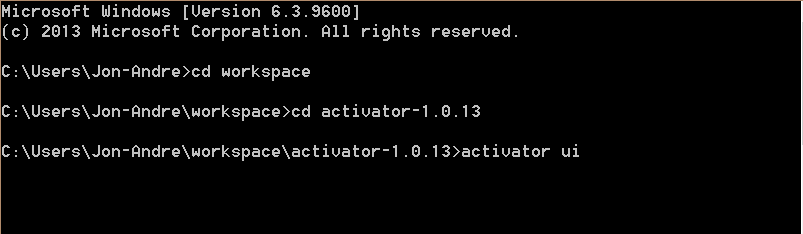
\includegraphics[scale=0.8]{guide/activator1.png} 
\end{center}
The graphical user interface should then open automatically in a browser view. If this doesn't happen check the terminal for error messages.

\paragraph{}
In the right sidebar navigate to the folder where you have cloned StedR\_server from GitHub. Click choose. Now the program is starting to compile, and the server will try to run as a local instance on \href{http://127.0.0.1:9000}{localhost port 9000}. 
\begin{center}
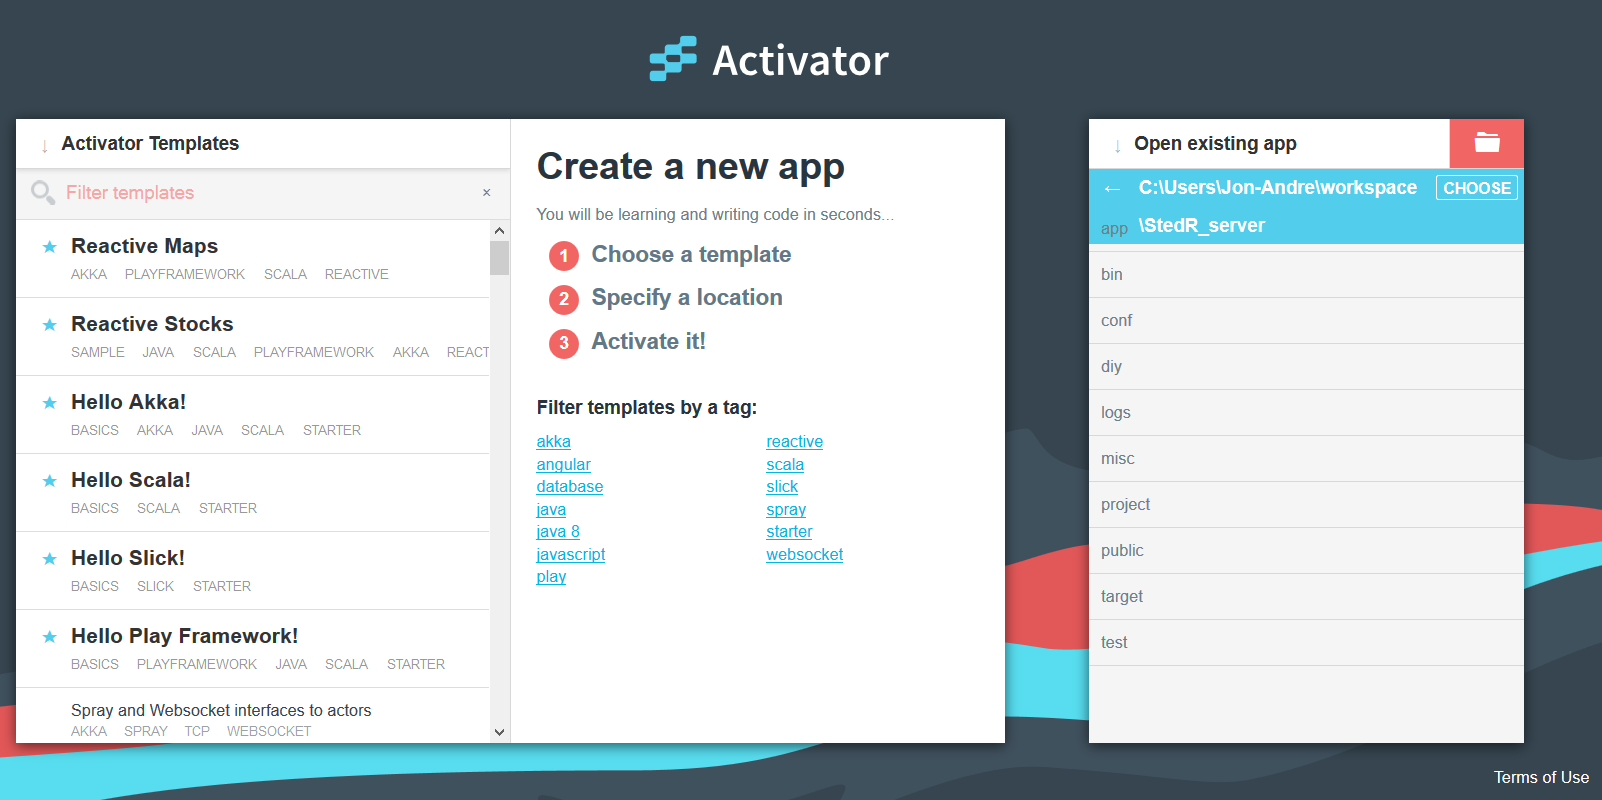
\includegraphics[scale=0.4]{guide/activator2.png} 
\end{center}

Notice that Typesafe Activator itself is running on port 8888. During the compiling of the system problems may occur. Often this is related to a mismatch between Typesafe and Java, for example an updated version of Java and an outdated version of Typesafe often leads to issues. If the program is compiled successfully, something like this should appear at localhost: 

\begin{center}
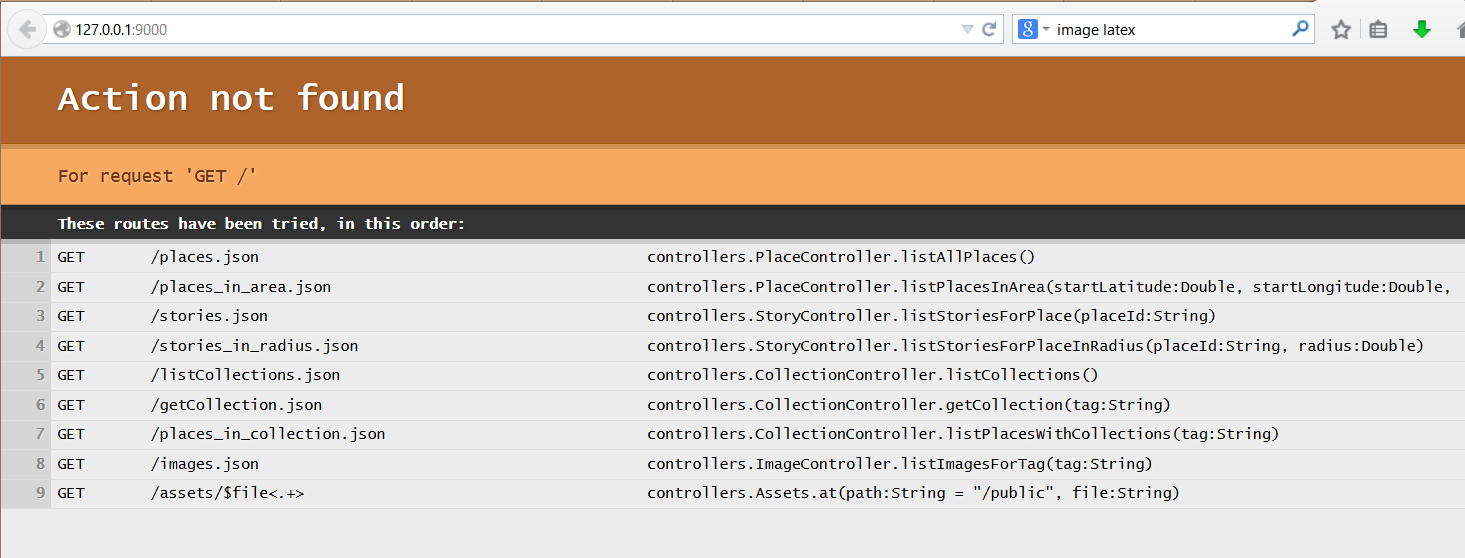
\includegraphics[scale=0.5]{guide/activator3.png} 
\end{center}

If you already have tried importing the folder with the source code to an editor like Eclipse, you may have noticed a lot of errors appears. To import the program and its dependencies as a project: In the left sidebar of Typesafe, click on Code, then the gear-icon. Here you can choose between IntelliJ and Eclipse, and Typesafe will then generate project files and guide you through how to open the program as a project. 
\begin{center}
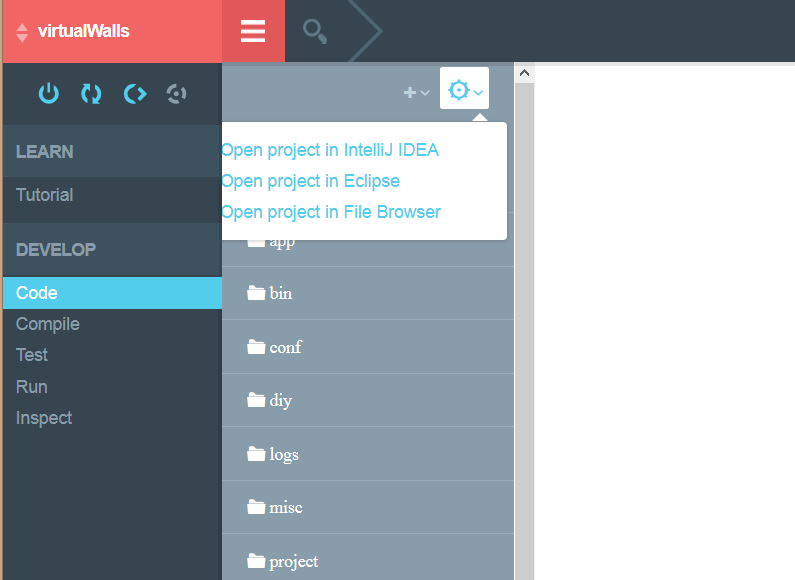
\includegraphics[scale=0.6]{guide/activator4.png} 
\end{center}
Now you should have a running instance of the server locally, and you're also ready to code. 

\paragraph{}

In Eclipse you will get an overview of the different source files and source packages. In the \texttt{Controllers} package you will find \texttt{controllers} that take care of identifying queries (sent as an URL), creating \texttt{Retrievers} that process the queries and at last returning a response to the query. All of the  \texttt{Controllers} are written by former Stedr-developers, but all of the  \texttt{Controllers} extends a  \texttt{Controller} from the Play Framework.

\begin{center}
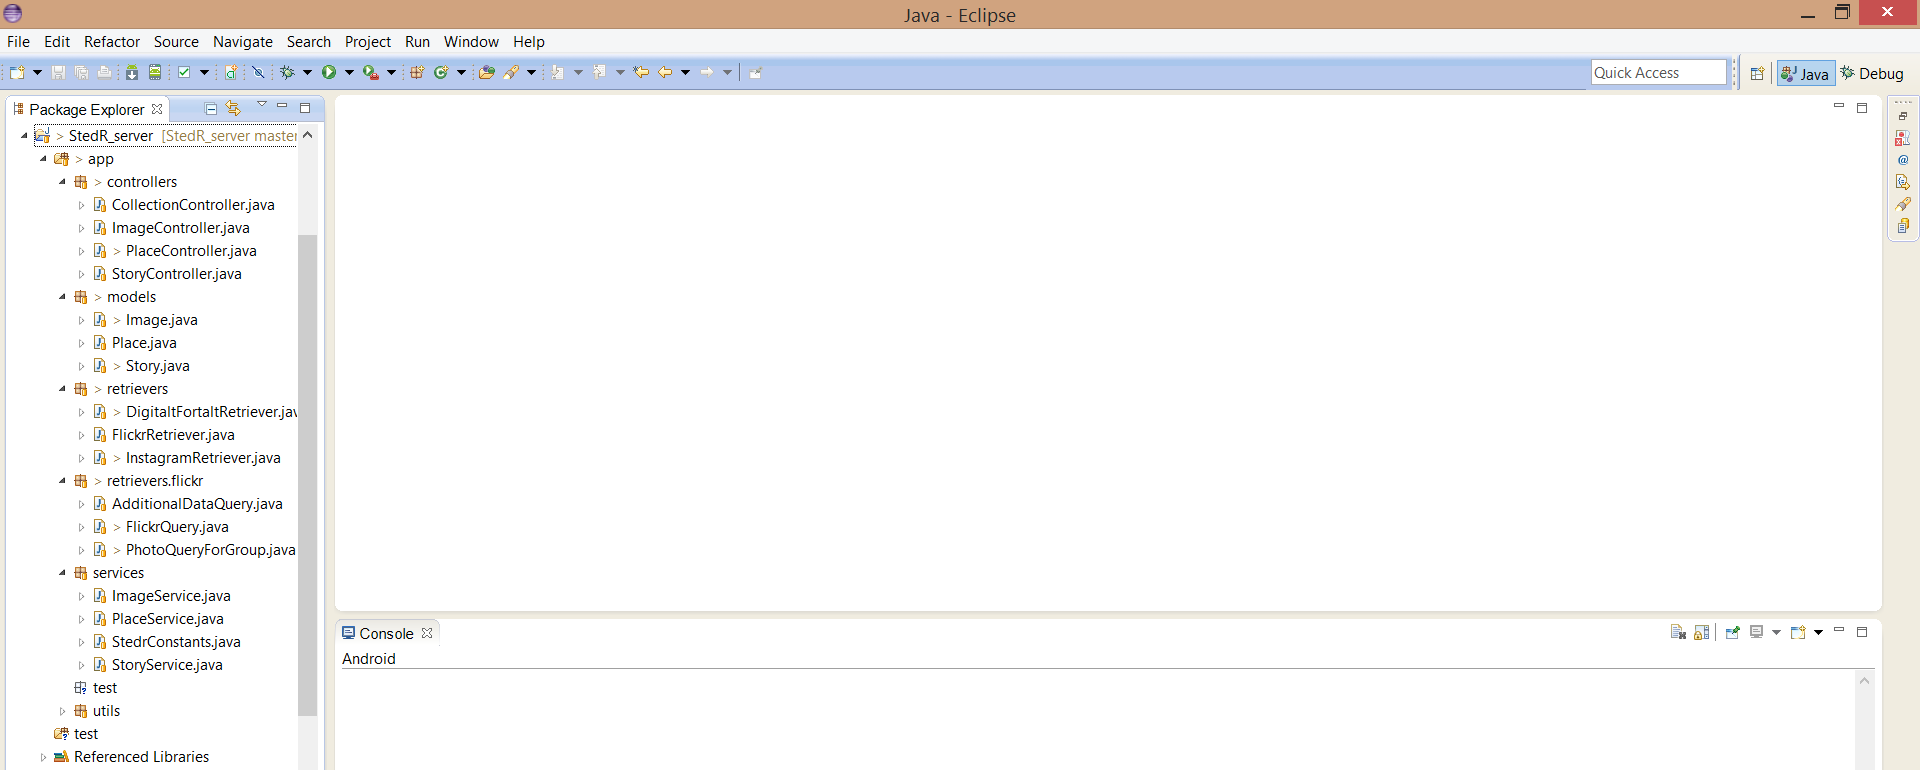
\includegraphics[scale=0.4]{guide/eclipse1.png} 
\end{center}

Now, let's create a controller for our example application:


\begin{center}
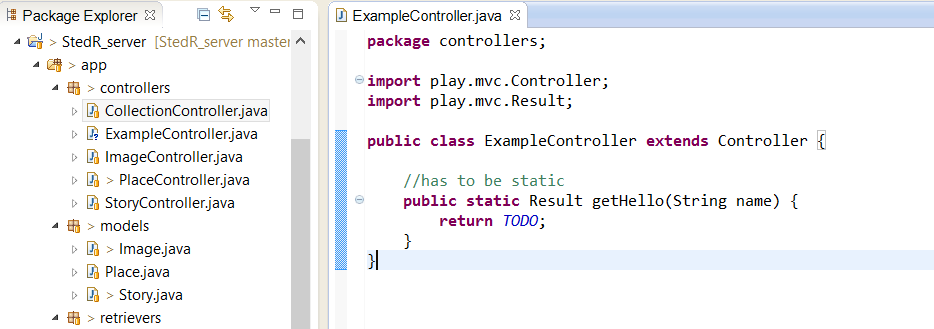
\includegraphics[scale=0.7]{guide/eclipse2.png} 
\end{center}

We ask for a parameter called \texttt{name} which naturally is the name you want to be displayed in the smartphone-application. To pass a parameter you have to edit the file called \texttt{routes} in the conf-folder, the passing is done directly from the smartphone application.

\begin{center}
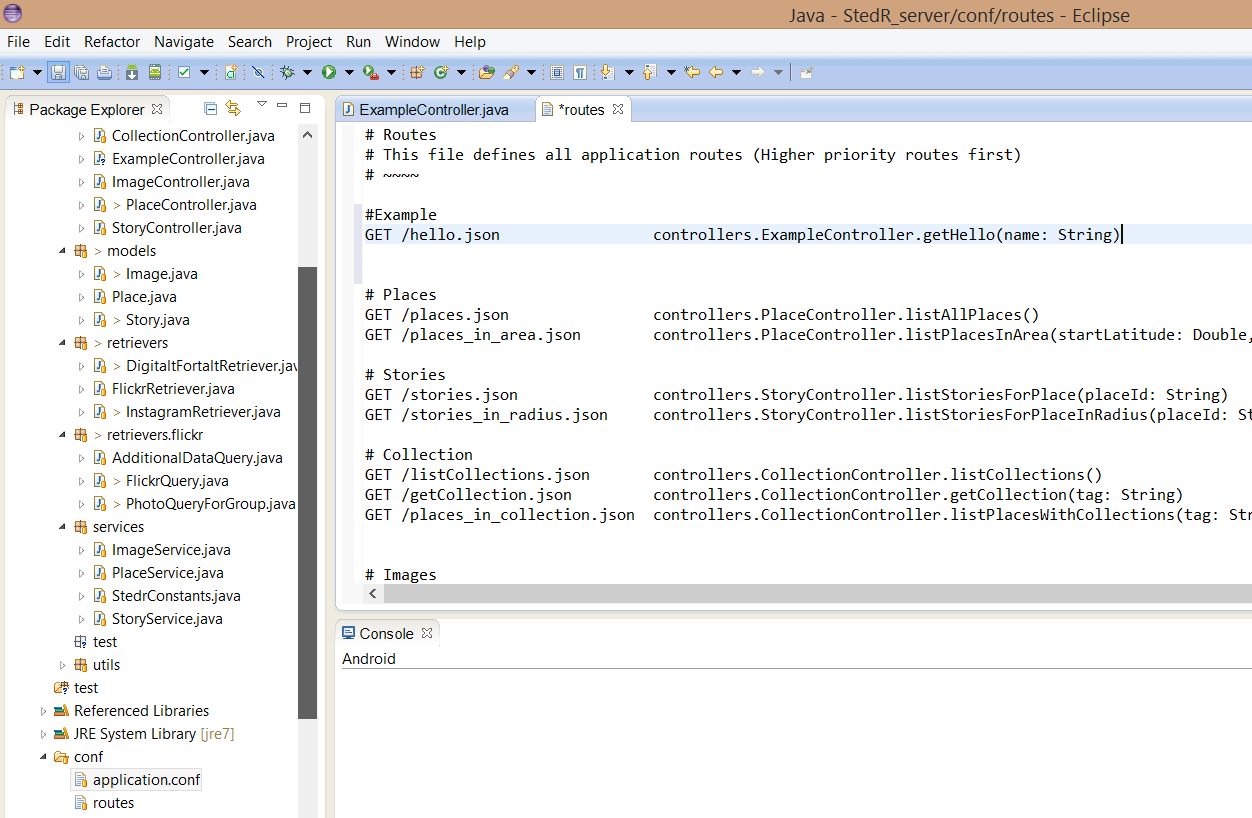
\includegraphics[scale=0.5]{guide/eclipse3.png} 
\end{center}

It would now have been possible to create a \texttt{retriever} directly, but we won't do that. In the services folder there are three files ending with  \texttt{Service.java}. These files are interfaces, and the reasoning behind them is that it should be easy to add or change services. As of now stories are provided by Digitalt Fortalt, so we have a \texttt{DigitaltFortaltRetriever.java} which implements \texttt{StoryService.java} That way we can change the content provider to Wikipedia by creating a new retriever \texttt{WikipediaRetriever.java} which implements \texttt{StoryRetriever.java} A lot of code would then have to be written in order to get the fictional \texttt{WikipediaRetrever.java} functional. Back to the example we will therefore create an ExampleService. 

\begin{center}
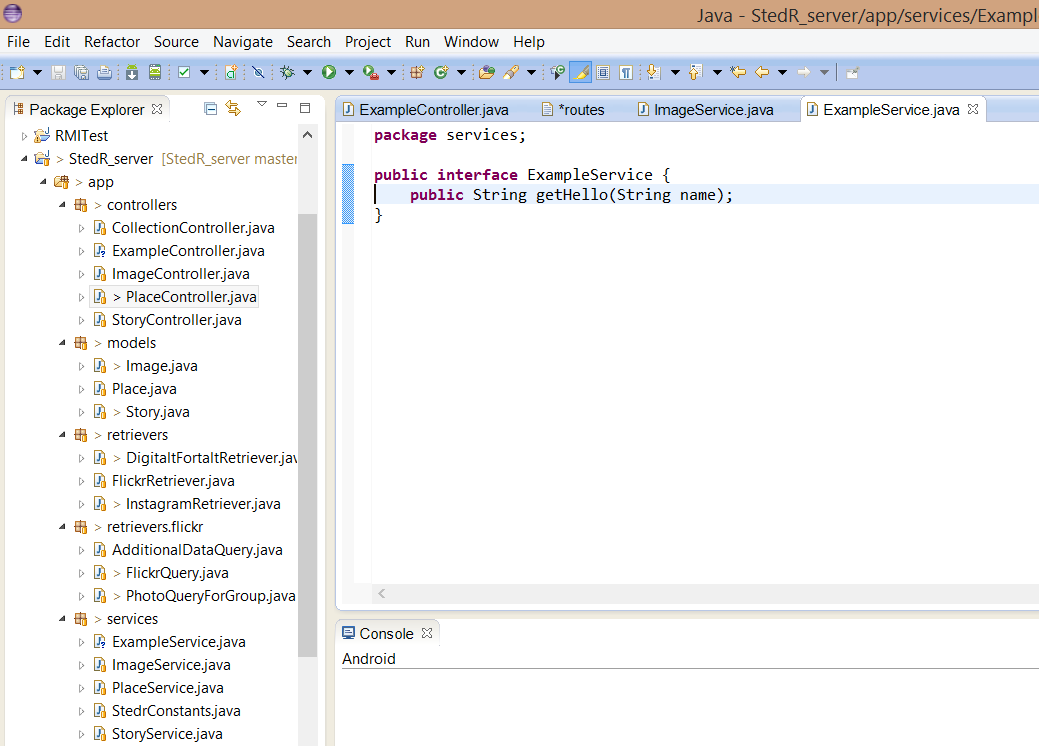
\includegraphics[scale=0.7]{guide/eclipse4.png} 
\end{center}

Now we're ready to implement the \texttt{HelloRetriever}

\begin{center}
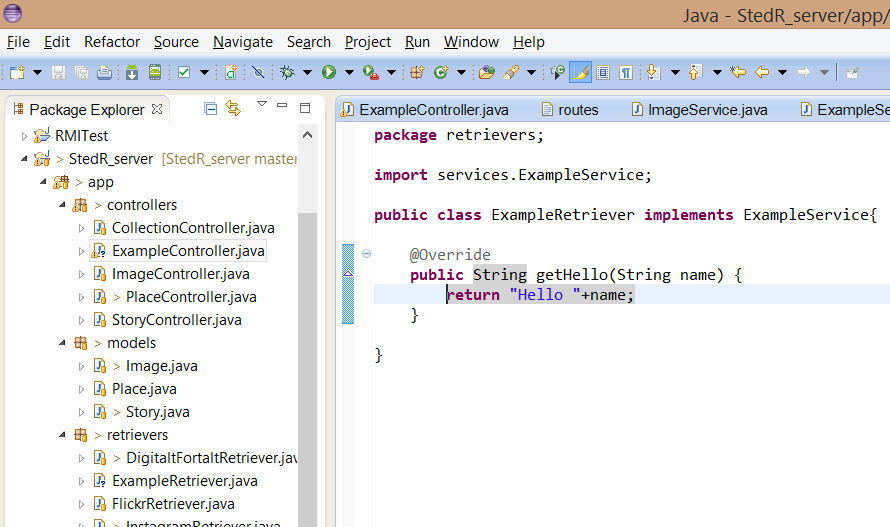
\includegraphics[scale=0.7]{guide/eclipse5.png} 
\end{center}

After the \texttt{HelloRetriever.java} the last thing that needs to be completed is the ExampleController which was created in the beginning of the example

\begin{center}
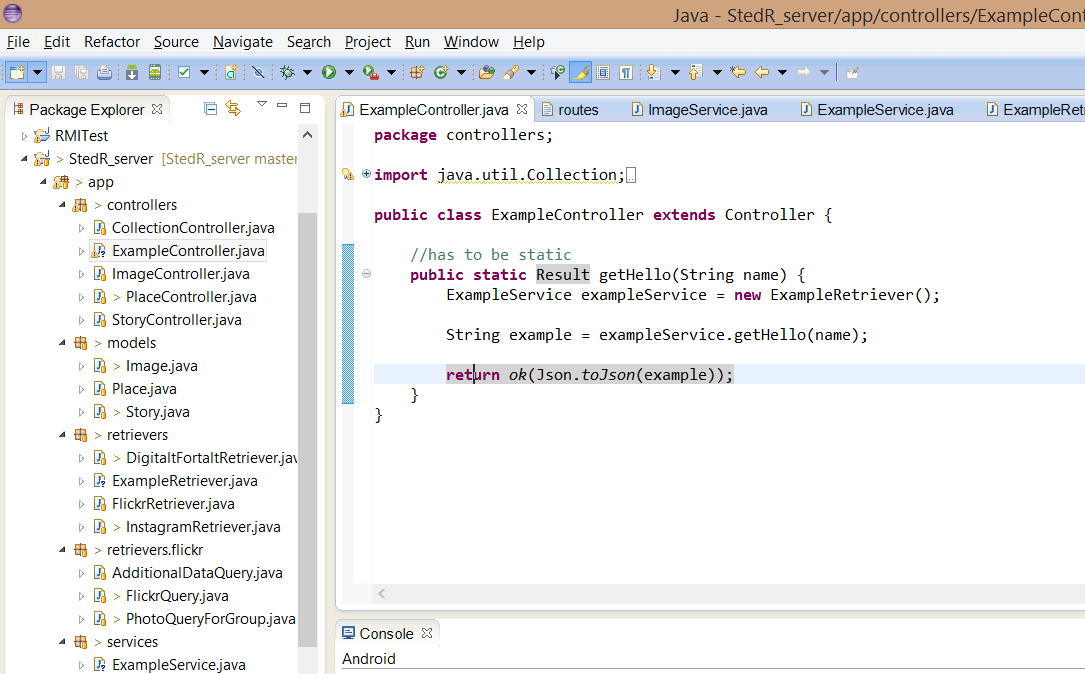
\includegraphics[scale=0.6]{guide/eclipse6.png} 
\end{center}

This concludes in a server which will respond with \texttt{Hello World} if  \texttt{World} is passed as a parameter. To see this, the system has to be recompiled in TypeSafe Activator. After recompiling open \href{http://127.0.0.1:9000}{localhost port 9000}, there you should see:

\begin{center}
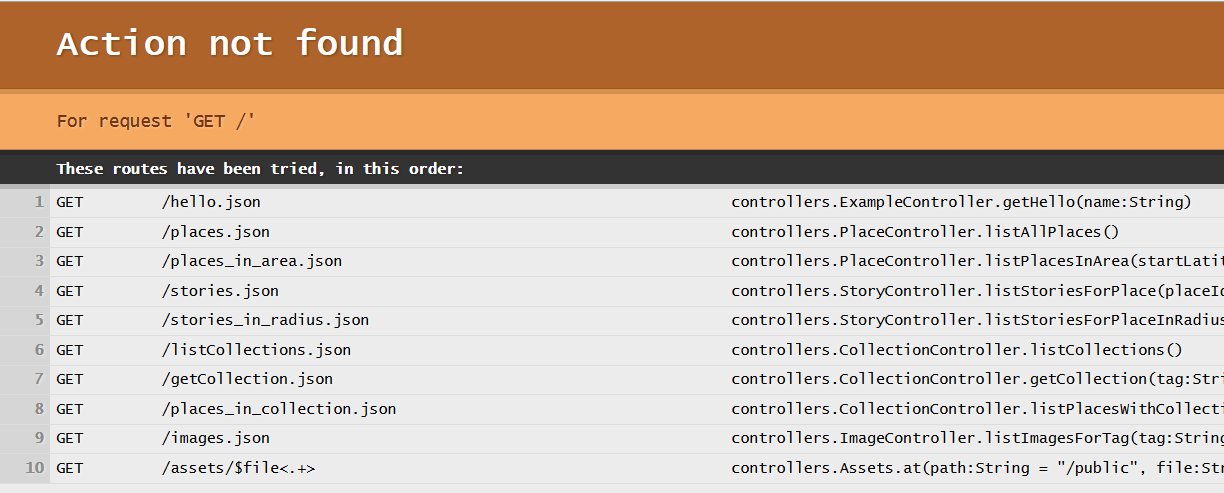
\includegraphics[scale=0.6]{guide/localhost.png} 
\end{center}

If this is correct,  \href{http://127.0.0.1:9000/hello.json?name=world}{http://127.0.0.1:9000/hello.json?name=world} should give:

\begin{center}
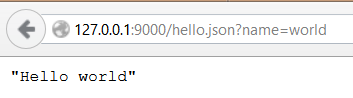
\includegraphics[scale=0.8]{guide/completed.png} 
\end{center}

Normally you would commit this to the git-repository on GitHub, and if the new functionality is to be a part of the running server it should also be committed or deployed to Heroku. This is done by pushing the server to \texttt{git@heroku.com:stedr-beta.git}. Note that in order to push to the server directly, you will need contributor access to stedr-beta.herokuapp.com. If this isn't available or provided upon request you can create a new Heroku instance, but then the request URL destinations have to be changed in the smartphone application.

\textbf{Remember to add the API-keys to the \texttt{StedrConstants.java}. These must ONLY be added to private repositories!!! Also, since almost all of them are owned by members of former dev-teams they may become invalid without notice}:


\texttt{// this apikey belongs to: chrisfro@stud.ntnu.no} \\
\texttt{public static final String FLICKR\_API\_KEY = } \\
\hspace*{4em}\texttt{"cd04f142470e7de7c992b3a3b140f636";} \\
\texttt{public static final String STEDR\_GROUP\_ID =} \\ 
\hspace*{4em}\texttt{"2297124\%40N25"; // escaped} \\
\texttt{this access token belongs to: knut.nerga@gmail.com} \\
\texttt{public static final String INSTAGRAM\_ACCESS\_TOKEN =} \\ 
\hspace*{4em}\texttt{"623771306.1fb234f.09aa9355cc8e469f8839d18385f719d5";} \\
\texttt{// this access token belongs to: Jacqueline Floch} \\
\texttt{public static final String DIMU\_API\_KEY =} \\ 
\hspace*{4em}\texttt{"h\_LUmtZbSAC9CqsDzsuzgg";} \\
\texttt{// these access tokens belongs to: Tor Barstad} \\
\texttt{public static final String SOUNDCLOUD\_CLIENT\_ID =} \\ 
\hspace*{4em}\texttt{"737095f8e223d83af9b88a9b48d90ea9";} \\
\texttt{public static final String SOUNDCLOUD\_CLIENT\_SECRET =} \\ 
\hspace*{4em}\texttt{"c559b568bfa50272ff18bcb27a87fa65";} \\

\subsection{Front-end}

The frontend is developed using Appcelerator Titanium.  Similar to the backend, the source code itself is maintained on a GitHub account provided by Sintef called TagCloud. Before continuing this means that a couple of prerequisites has to be fulfilled by the developer.

\paragraph{The developer should have:}
\begin{itemize}
\item A working GitHub-account 
\item A working Appcelerator-account 
\item Installed git
\item Cloned TagCloud/VirtualWall with the help of Git from GitHub.
\item An Android or iOS device
\end{itemize}  

Note that you need a to install the sync software for your device and make sure you have USB debugging enabled. It is also important to note that you need a Mac in order to build the program for iOS devices. Android or iOS device is not required, since it is possible to use an emulator. 

\paragraph{}

Download \href{http://www.appcelerator.com/titanium/}{Appcelerator Titanium}.

Install titanium by following the installation wizard. When titanium is finished installing, open it. Titanium will ask you to choose a workspace location, where your projects will be stored. You then have to log in with your Appcelerator-account.

Titanium will then most likely attempt to install software development kit (SDK) for Android. If it does not, you can do so via the dashboard. Click the “Get Started” tab and scroll to “Configure Native SDKs”, click Android SDK and make sure it is updated. The Tizen and Blackberry deveopment kits are not necessary for this application.

If you have a Mac, you should be able to install the iOS SDK aswell. You need this if you are testing the application on an iOS device.

\begin{center}
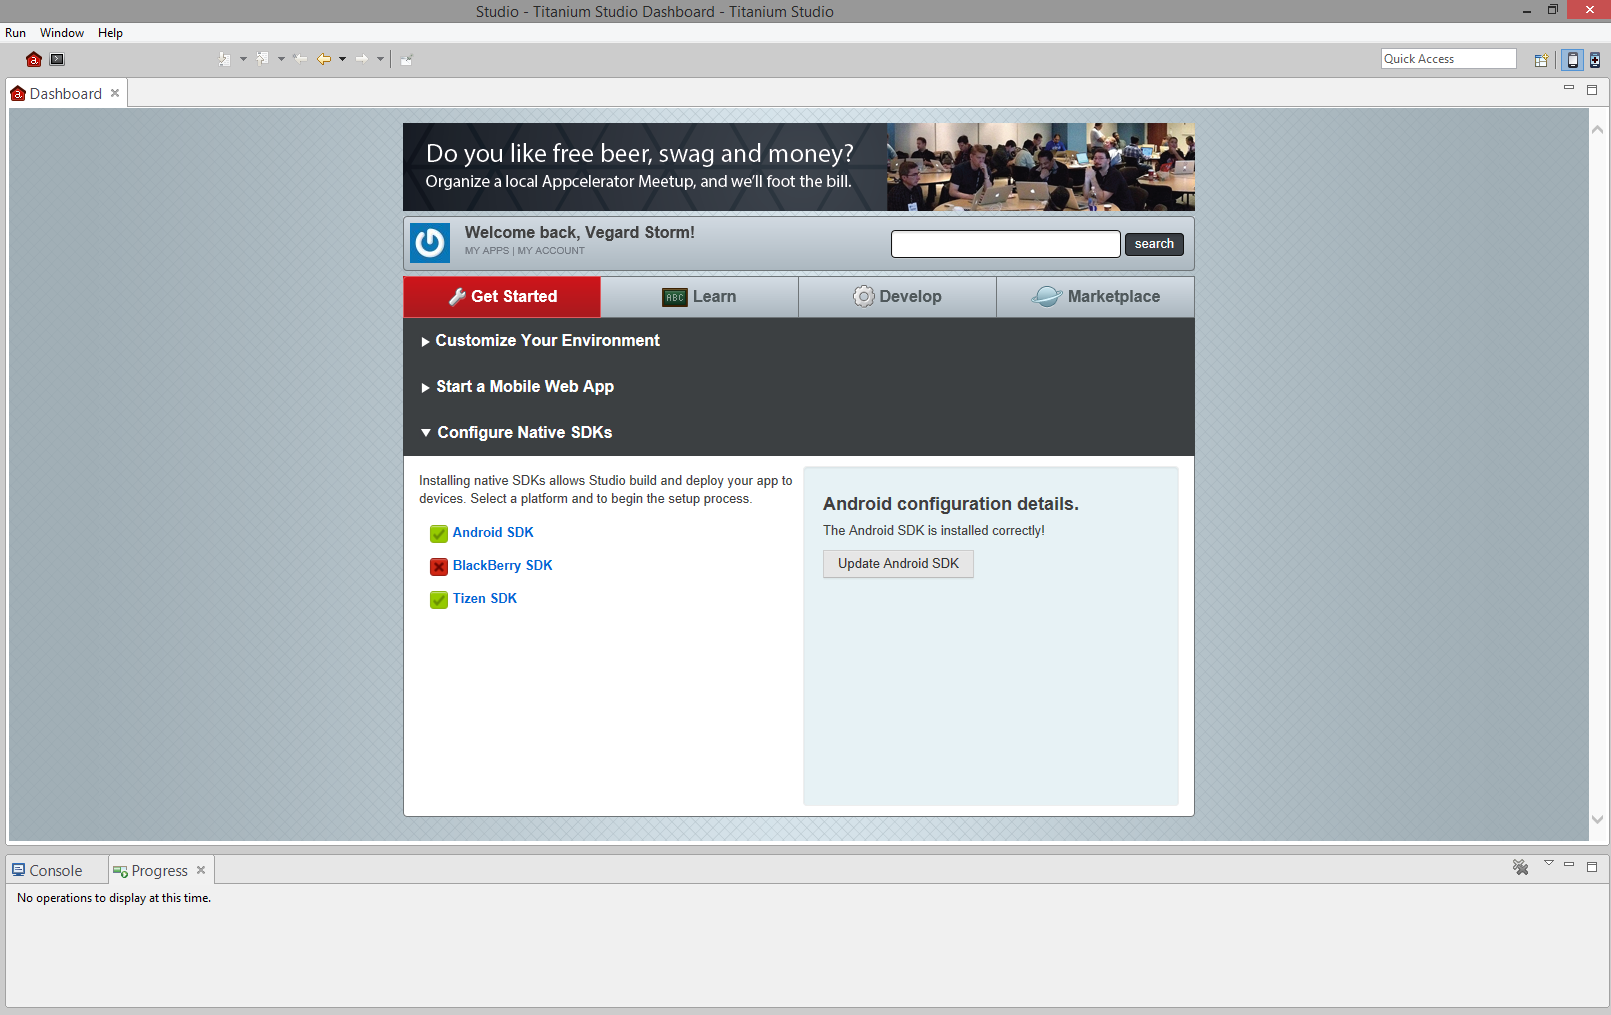
\includegraphics[scale=0.3]{guide/f1.png} 
\end{center}

Now we are ready to import the stedr project.
1. Right click in the project explorer and choose “Import”.
2. Choose the “Existing Folder as New Project”-option under “General” and press “Next”.

\begin{center}
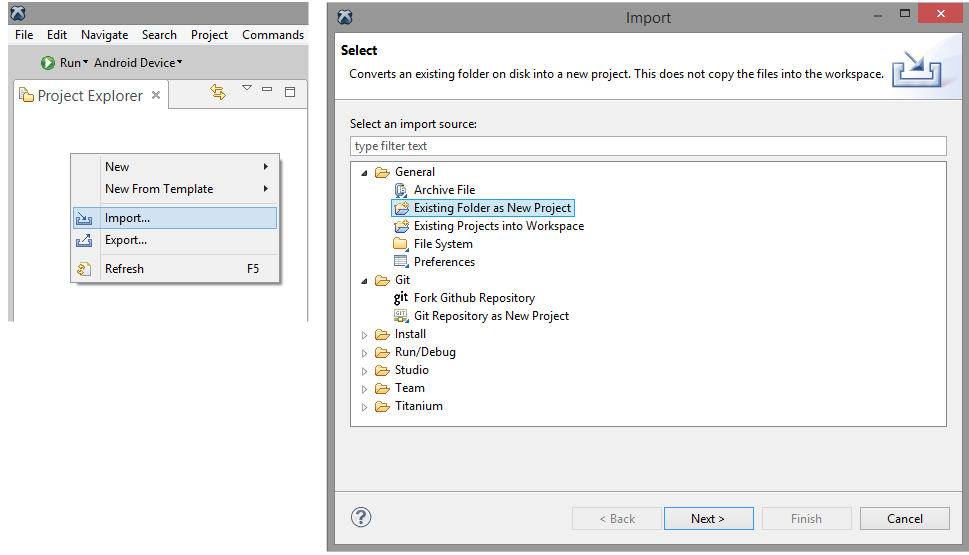
\includegraphics[scale=0.45]{guide/f2.png} 
\end{center}

3. Click browse and choose the folder where you downloaded stedr and press “OK”. 
Example: C:/Users/Vegard/Documents/GitHub/VirtualWall/stedr
4. Under “Project type” make sure Alloy is checked as primary and mobile is checked (This should happen automatically) and press “Finish” if everything is in order.

\begin{center}
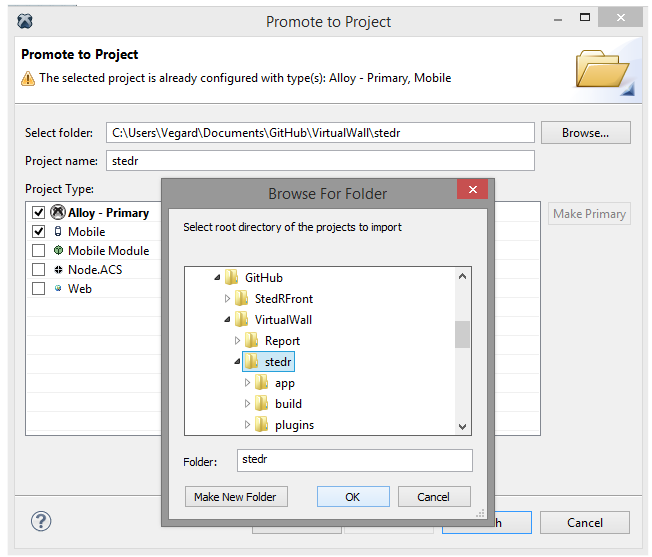
\includegraphics[scale=0.45]{guide/f3.png} 
\end{center}

We are now ready to code or run the project. It might benefial to try to run the program on your device or an emulator before you start coding. If you have already done what is explained in the prerequisites and connected your device to the PC via USB, your phone should show up in the list of devices as desplayed below. If it does, select it and click “Run”. However if it does not, make sure you have the synchronization software for your device installed, and that you have “USB debugging” enabled in your phone settings. If you have issues finding the “USB debugging” option on your phone, it may be because you do not have access to developer settings. The easiest way to figure out how to get access is to google “how to access developer options on *your device*“.

\begin{center}
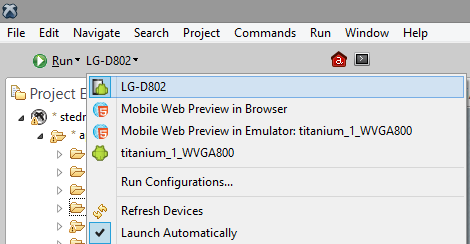
\includegraphics[scale=0.45]{guide/f4.png} 
\end{center}

\paragraph{Emulator:}
It is possible to run the program on the official Android emulator, but it has some performence issues. An alternative emulator is the \href{https://shop.genymotion.com/index.php?controller=order-opc}{Genymotion}. Note that this emulator has some restrictions when asking for a free license, so make sure not to break their term of service. 

Genymotion does not support Google Apps (i.e Google Map Servce) which is needed to run stedr. To install Google Apps on Genymotion, see this \href{https://www.youtube.com/watch?v=iCRNqCXGNK0}{screencast}. Before continuing it is also practical to add adb to the enviromental path, so that adb is accessible directly in the terminal. On Windows you can locate adb.exe under the folder platform-tools where you have installed the Android SDK. 

With Genymotion started (the emulated device should be running) enter \texttt{adb install -r stedr.apk}. It is easiest to do this from the builder folder where, but you can probably send the location of the apk as a parameter. Notice the -r parameter, this is for reinstalling an apk which becomes necessery to use if the apk already is installed at the emulated device.

\begin{center}
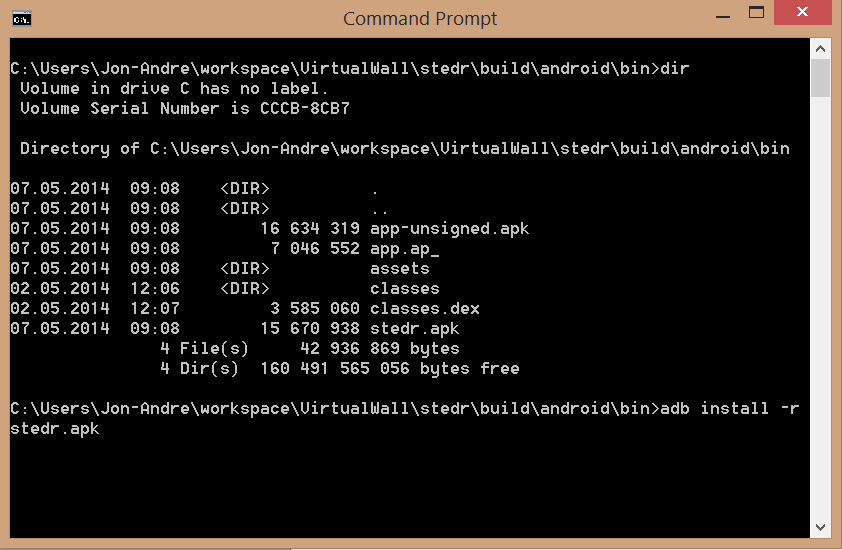
\includegraphics[scale=0.7]{guide/f45.png} 
\end{center}

\paragraph{Structure in Titanium alloy:}
if you explore your newly added stedr project in the project explorer you will notice that under the app folder there are a nouber of subfolders.

\begin{wrapfigure}{l}{0.5\textwidth}
\begin{center}
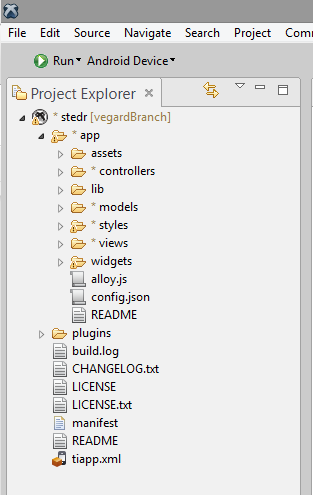
\includegraphics[scale=0.45]{guide/f5.png} 
\end{center}
\end{wrapfigure}

The views-, styles- and controllers-folders are the ones you will be working with the most.

Views:
This folder contains an XML-file for every view and the basic structure of it containing different UI-elements. Each element with an “id” will also get the properties assigned to it in the corresponding styles-file and controller-file.

Styles:
This is a folder of TSS-files that are used to design elements used in the corresponding XML-file based on “id”.

Controllers:
This folder is where the JavaScript classes for the different views are stored and where you can add code that affect the corresponding view. You add new UI elements,  event listeners, functions and more to achieve the desired functionality and design.


Additionally we have the assets folder, where media like pictures are stored; the lib folder, where you store relevant imported libraries; the models folder, where you can create models that are useful when for instance converting a string into an object; the widgets folder, where imported pre-made UI-elements are stored.


\paragraph{Coding Example}
In this example we assume that you have completed the backend example and uploaded it to the server stedr-beta.herokuapp.com.

We will be creating a view that cointains a label with the value that we retrieve from the server stedr-beta.herokuapp.com/hello.json?name=world. If done right, the text “Hello World” should be deplayed on the screen when opening this view. 

1. Begin by creating a new devTest.xml-file in the “views”-folder, a devTest.tss-file in the “styles”-folder and a devTest.js-file in the “controllers”-folder.

\begin{center}
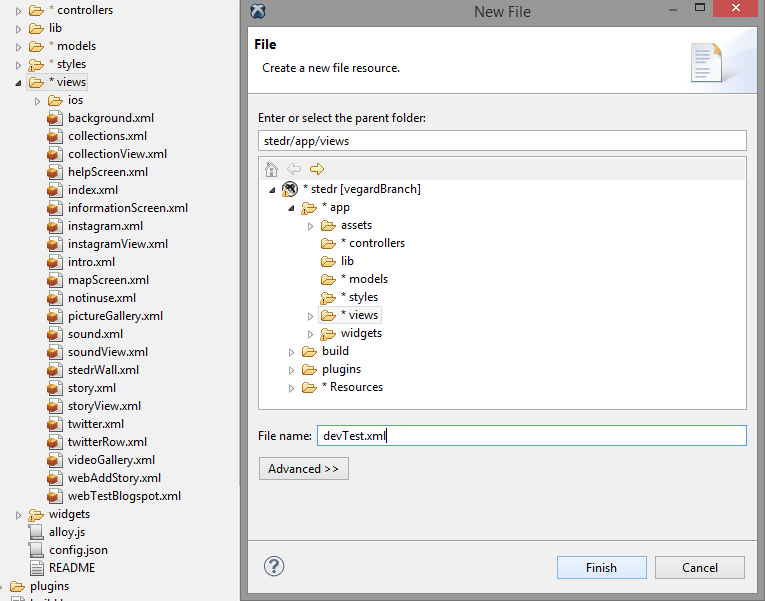
\includegraphics[scale=0.45]{guide/f6.png} 
\end{center}

2. Creating the XML-file for the view. This is the basic structure of the UI elements. You can also add some properties to the different elements.

\begin{center}
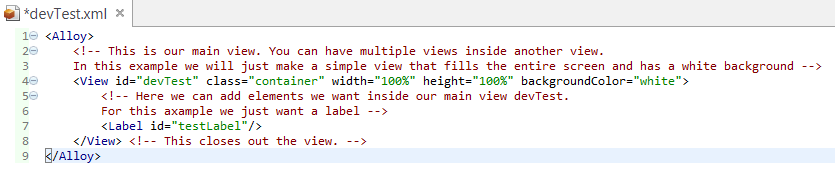
\includegraphics[scale=0.45]{guide/f7.png} 
\end{center}

2. Creating the TSS-file for the view. The purpose of this file is mainly to stylize UI-elements that are used more than once in the XML-file. Even though a TSS-file is not necessary for a simple view like is this and can be done easily in either the XML- or the JavaScript-file example, here is how you would stylize the label using TSS: 

\begin{center}
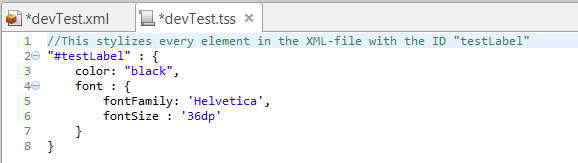
\includegraphics[scale=0.45]{guide/f8.png} 
\end{center}

3. Creating the JavaScript-file. This is where we retrieve the information from the server, aswell as set the text of the label.

\begin{center}
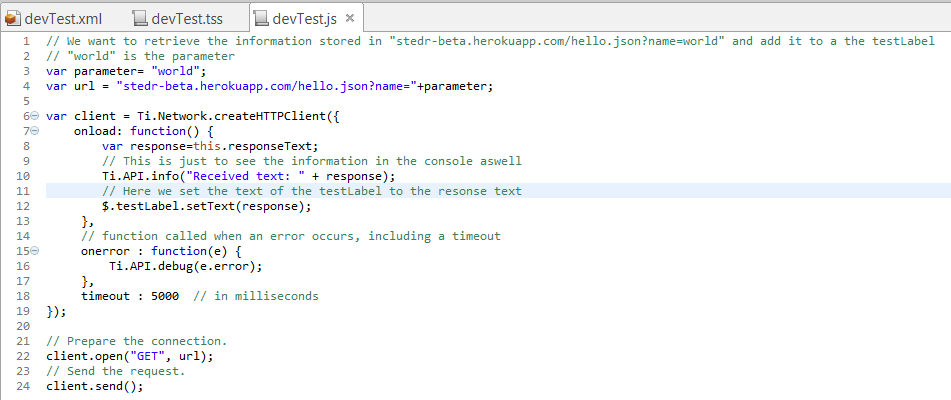
\includegraphics[scale=0.45]{guide/f9.png} 
\end{center}

Now all we have to do is open this view where we want it. For test purposes i will in this exaple set it to open automatically when you open the app. To do this, we have to go into the index.js file under controllers. Every window/view opens or closes through this class because this is where the window stack is. To make sure the test view is shown automatically, scroll down to the bottom of index.js and add it right above \$.index.open() as shown below:

\begin{center}
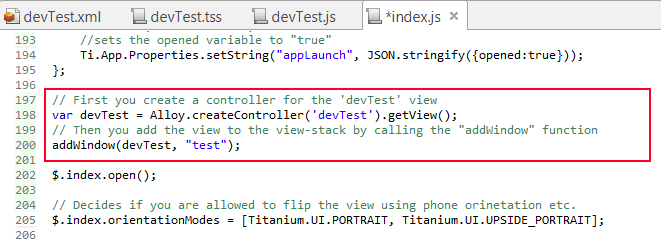
\includegraphics[scale=0.45]{guide/f10.png} 
\end{center}
Now if you save and run you should see something like this when you start the application on your phone:

\begin{wrapfigure}{l}{0.5\textwidth}
\begin{center}
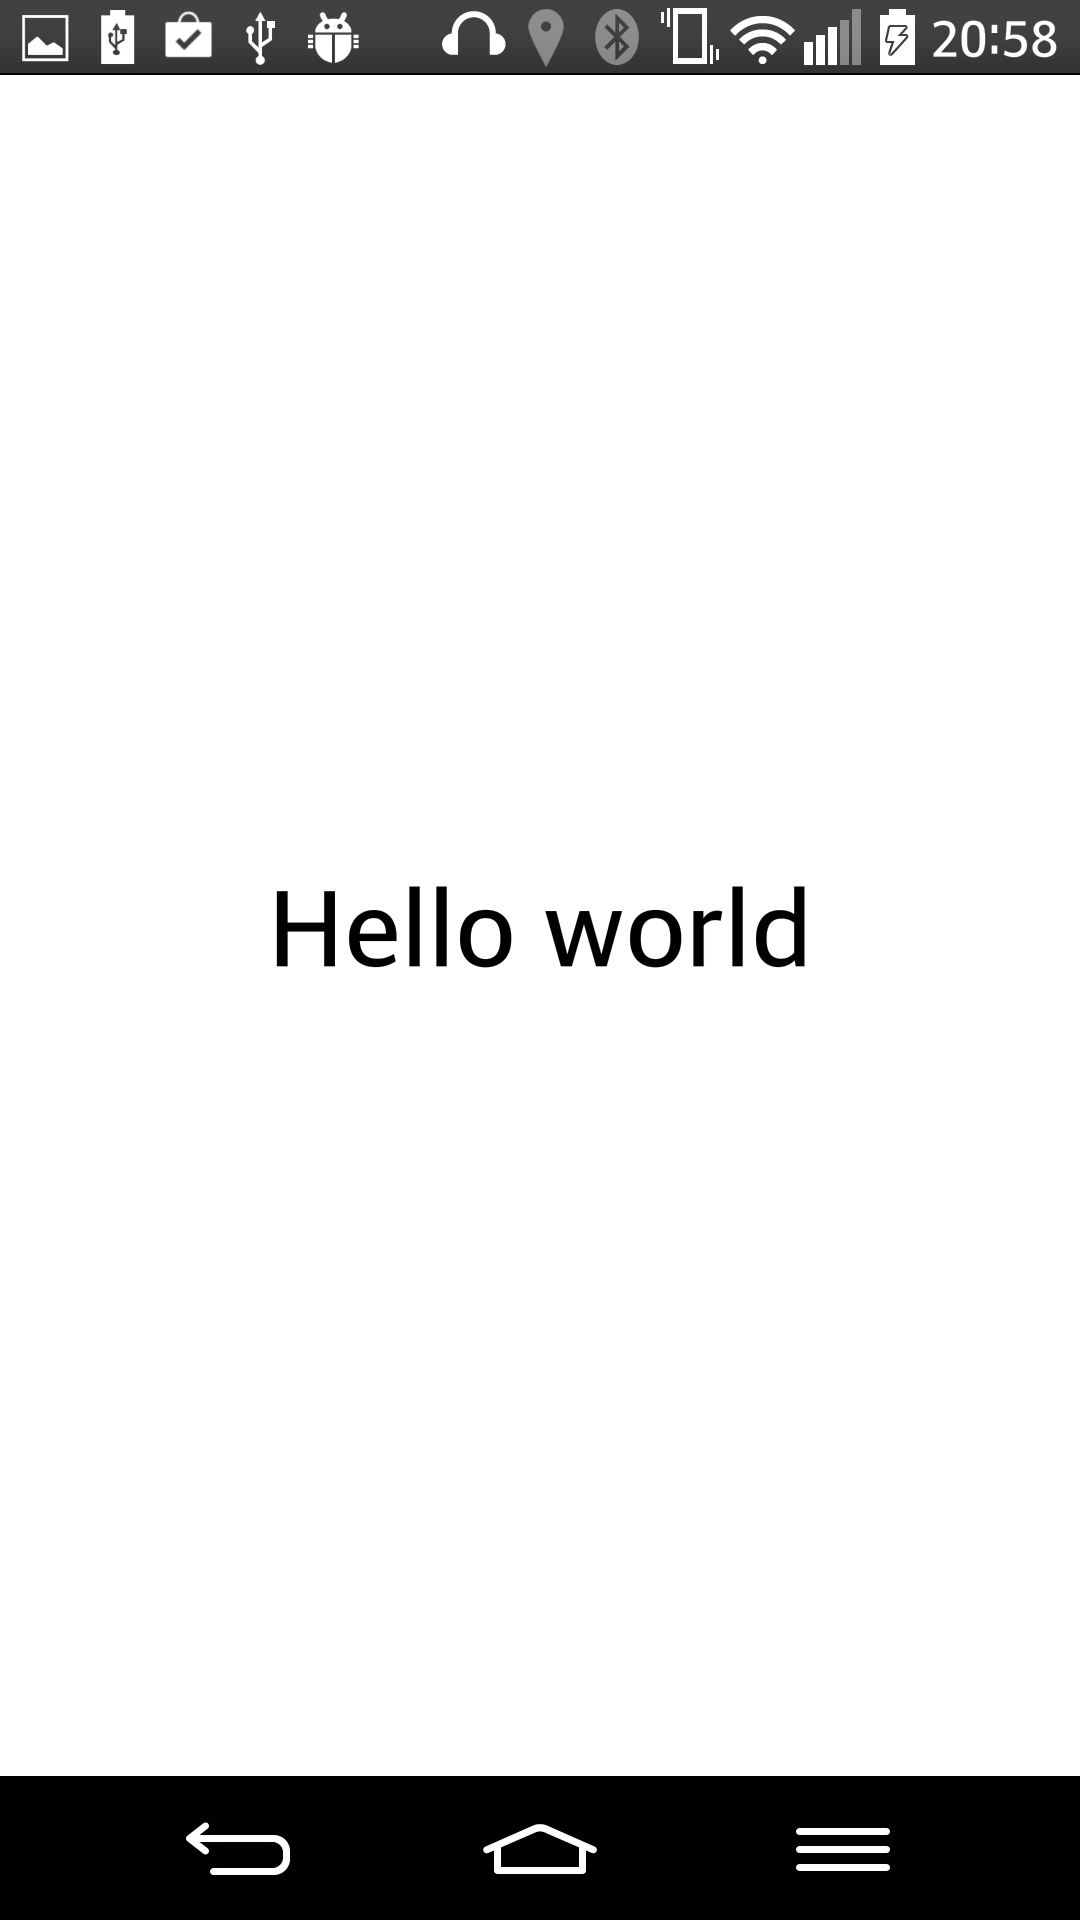
\includegraphics[scale=0.15]{guide/f11.png} 
\end{center}
\end{wrapfigure}

We have now gone over the basics of how to create a view aswell as retrieving information from the server. To further understand how to develop stedr using Titanium, looking at and understanding the previous code is essential. The documentation available on the \href{http://docs.appcelerator.com/titanium/3.0/}{Appcelerator website} is also extremely helpful when learning about Titanium:
